\documentclass[a4paper,12pt]{article}
% -------------------------------------------------
% Configuração de página
% -------------------------------------------------
\usepackage[a4paper,top=3cm,bottom=2cm,left=3cm,right=2cm]{geometry}
% -------------------------------------------------
% Codificação e idioma
% -------------------------------------------------
\usepackage[T1]{fontenc}
\usepackage[utf8]{inputenc}
\usepackage[english,brazil]{babel}
\usepackage{mathptmx}
% -------------------------------------------------
% Pacotes matemáticos e fontes
% -------------------------------------------------
\usepackage{amsmath}
\usepackage{amsfonts}
\usepackage{amstext}
\usepackage{mathptmx}
% -------------------------------------------------
% Formatação geral
% -------------------------------------------------
\usepackage{indentfirst}
\usepackage{microtype}
\usepackage{setspace}
\onehalfspacing
\setlength{\parindent}{1.25cm}
\setlength{\parskip}{0pt}
% -------------------------------------------------
% Gráficos, tabelas e quadros
% -------------------------------------------------
\usepackage{graphicx}
\usepackage{graphics}
\usepackage{pgfplots}
\pgfplotsset{compat=1.18}
\usepackage{float}
\usepackage{booktabs}
\usepackage{array}
\usepackage{tabularx}
\usepackage{longtable}
\usepackage{multirow}
\usepackage{makecell}
\usepackage{threeparttable}
\usepackage[table,xcdraw]{xcolor}
\usepackage[format=hang]{caption}
\captionsetup[quadro]{justification=centering}
% -------------------------------------------------
% Quadros (ambiente próprio)
% -------------------------------------------------
\usepackage{tocloft}
\usepackage{caption}
\floatstyle{plaintop}
\newfloat{quadro}{htbp}{loq}
\floatname{quadro}{Quadro}
\newcommand{\listofquadros}{
    \listof{quadro}{Lista de Quadros}
}
% -------------------------------------------------
% Outros pacotes
% -------------------------------------------------
\usepackage{enumerate}
\usepackage{nomencl}
\usepackage{color}
\usepackage{verbatim}
\usepackage{hyperref}
\usepackage[alf]{abntex2cite}
\usepackage{colortbl}
\usepackage{tcolorbox}
\usepackage{fancyhdr}
\usepackage{appendix}
\usepackage{multicol}
\usepackage{adjustbox}
\usepackage{wasysym}
\usepackage{pdflscape}
\newcommand{\fonte}[1]{\par\noindent\footnotesize Fonte: #1}
\newcommand{\nota}[1]{\par\noindent\footnotesize Nota: #1}
\newcommand{\celula}[1]{\makecell[l]{#1}}
% -------------------------------------------------
% Listagem de código-fonte
% -------------------------------------------------
\usepackage{listings}
\renewcommand{\lstlistingname}{Código}
\renewcommand{\lstlistlistingname}{Lista de Códigos}
% -------------------------------------------------
% Acentuação em listagens
% -------------------------------------------------
\lstset{
    basicstyle=\ttfamily\small,
    numbers=left,
    numberstyle=\tiny,
    stepnumber=1,
    numbersep=8pt,
    frame=single,
    breaklines=true,
    tabsize=4,
    showstringspaces=false,
    captionpos=b,
    keywordstyle=\color{blue},
    commentstyle=\color{green!50!black},
    stringstyle=\color{red!70!black}
}
\lstset{
    basicstyle=\ttfamily\small,
    numbers=left,
    numberstyle=\tiny,
    stepnumber=1,
    numbersep=8pt,
    frame=single,
    breaklines=true,
    tabsize=4,
    showstringspaces=false,
    captionpos=b,
    keywordstyle=\color{blue},
    commentstyle=\color{green!50!black},
    stringstyle=\color{red!70!black},
    literate=
      {á}{{\\'a}}1 {à}{{\\\`a}}1 {ã}{{\\\~a}}1 {â}{{\\^a}}1
      {é}{{\\'e}}1 {ê}{{\\^e}}1
      {í}{{\\'i}}1
      {ó}{{\\'o}}1 {õ}{{\\\~o}}1 {ô}{{\\^o}}1
      {ú}{{\\'u}}1
      {ç}{{\c{c}}}1
      {Á}{{\\'A}}1 {À}{{\\\`A}}1 {Ã}{{\\\~A}}1 {Â}{{\\^A}}1
      {É}{{\\'E}}1 {Ê}{{\\^E}}1
      {Í}{{\\'I}}1
      {Ó}{{\\'O}}1 {Õ}{{\\\~O}}1 {Ô}{{\\^O}}1
      {Ú}{{\\'U}}1
      {Ç}{{\c{C}}}1
}
\usepackage{lipsum}
% -------------------------------------------------
% Documento
% -------------------------------------------------
\begin{document}
% -------------------------------------------------
% Folha de rosto
% -------------------------------------------------
\begin{titlepage}
    \thispagestyle{empty}
    \begin{center}
        % Logos
        \begin{minipage}{0.22\textwidth}
            \centering
            \includegraphics[width=0.9\linewidth]{figuras/logo\_ufs.png}
        \end{minipage}
        \hspace{1.5cm}
        \begin{minipage}{0.22\textwidth}
            \centering
            \includegraphics[width=0.9\linewidth]{figuras/logo\_ppgdem.png}
        \end{minipage}
        \par
        \vspace{1.2cm}
        % Instituições
        {\large UNIVERSIDADE FEDERAL DE SERGIPE\par}
        {\large UNIVERSIDADE FEDERAL DO RIO GRANDE DO NORTE\par}
        \vspace{0.5cm}
        {\large PROGRAMA DE PÓS-GRADUAÇÃO EM DEMOGRAFIA\par}
        {\large DOUTORADO INTERINSTITUCIONAL EM POPULAÇÃO,\par}
        {\large ESTATÍSTICAS SOCIAIS E POLÍTICAS PÚBLICAS\par}
        \vspace{3cm}
        % Nome do aluno
        {\large \textbf{Andrés Ignácio Martínez Menéndez}\par}
        \vspace{3cm}
        % Título
        {\Large \textbf{Técnicas Demográficas II}\par}
        \vspace{0.6cm}
        {\large Trabalho de População Estável\par}
        \vfill
        % Local e data
        {\small Aracaju (SE)\par}
        {\small Setembro de 2026\par}
    \end{center}
\end{titlepage}
    \clearpage
\newpage
\pagenumbering{arabic}


\section{Introdução}

A dinâmica de uma população resulta da interação entre fecundidade, mortalidade e migração. Quando as funções de fecundidade e mortalidade por idade permanecem constantes e se admite uma população fechada à migração, a distribuição etária converge, no longo prazo, para uma estrutura estável. Nessa condição, a população passa a apresentar composição etária invariável e crescimento a uma taxa constante, denominada taxa intrínseca de crescimento. O modelo de população estável permite, portanto, relacionar quantitativamente os padrões vigentes de reprodução e sobrevivência com suas consequências sobre o crescimento e a estrutura etária \cite{grupofoz2021,preston2001}.

A análise dessas relações requer a combinação de indicadores sintéticos e modelos estruturados por idade. As taxas específicas de fecundidade descrevem a intensidade da reprodução em cada grupo etário feminino e constituem a base para o cálculo da idade média à maternidade e das taxas bruta e líquida de reprodução. A Taxa Bruta de Reprodução (TBR) mede o número médio de filhas que uma mulher teria ao longo do período reprodutivo caso estivesse submetida às taxas de fecundidade observadas, sem considerar a mortalidade. A Taxa Líquida de Reprodução (TLR), por sua vez, incorpora a sobrevivência feminina até as idades reprodutivas. A partir dessas medidas, pode-se estimar a taxa intrínseca de crescimento por aproximação e, de forma mais rigorosa, mediante a solução numérica da equação de Euler--Lotka \cite{grupofoz2021,preston2001}.

Este trabalho tem como objetivo estimar indicadores de reprodução e analisar a população estável equivalente às condições demográficas do Distrito Federal em 2022. São estimadas a idade média à maternidade, a TBR, a TLR, a taxa intrínseca de crescimento e a taxa bruta de natalidade da população estável. A estrutura etária estável é obtida por duas abordagens: a formulação discreta de Euler--Lotka e a formulação matricial por grupos etários \cite{grupofoz2021,preston2001}. As estruturas resultantes são comparadas com a distribuição etária observada no Censo Demográfico de 2022.

Por fim, estima-se o momentum populacional em um cenário hipotético no qual a fecundidade alcança 
imediatamente o nível de reposição, enquanto a mortalidade permanece constante e não há migração. 
Esse procedimento permite mensurar quanto a população ainda aumentaria antes de atingir uma 
configuração estacionária, exclusivamente em razão da estrutura etária existente no início da 
projeção \cite{grupofoz2021,preston2001}. Todos os cálculos foram implementados no ambiente R, 
utilizando dados de população, nascimentos e óbitos referentes ao Distrito Federal. Todos os 
códigos utilizados, bem como os dados utilizados e os resultados, estão disponíveis no repositório 
do GitHub: \url{https://github.com/ammenendez/TD-02-trab02.git}.


\section{Dados e procedimentos gerais}

A análise foi realizada para o Distrito Federal, utilizando dados referentes ao ano de 2022. A escolha desse período permite compatibilizar as estatísticas vitais com os resultados do Censo Demográfico de 2022, reduzindo diferenças temporais entre os numeradores e denominadores empregados no cálculo das taxas. Foram utilizadas três fontes principais: o Sistema de Informações sobre Nascidos Vivos (SINASC), para os nascimentos segundo a idade da mãe e o sexo da criança; o Sistema de Informações sobre Mortalidade (SIM), para os óbitos segundo idade e sexo; e o Censo Demográfico de 2022, consultado por meio do Sistema IBGE de Recuperação Automática (SIDRA), para a população residente por idade e sexo \cite{datasussinasc2022,datasussim2022,ibge2022censo,ibgesidra9514}.

Os dados do SINASC foram selecionados segundo a residência da mãe, e não segundo o local de ocorrência do nascimento. Para o cálculo das taxas de fecundidade, foram considerados os sete grupos etários quinquenais compreendidos entre 15 e 49 anos. Os cinco nascimentos cujo sexo não estava informado foram redistribuídos entre os sexos masculino e feminino dentro do respectivo grupo etário da mãe, proporcionalmente à distribuição dos registros com sexo conhecido. Após o arredondamento, o complemento de cada total foi atribuído ao sexo masculino, garantindo a preservação do número total de nascimentos em cada faixa etária.

As populações femininas utilizadas como denominadores das taxas específicas de fecundidade foram obtidas da Tabela 9514 do SIDRA. Os grupos foram ordenados de 15--19 a 45--49 anos e associados às respectivas populações femininas. Para os cálculos de mortalidade e sobrevivência, foram construídas tábuas de vida abreviadas separadamente para homens e mulheres. Os óbitos com idade ignorada foram distribuídos proporcionalmente entre os grupos etários com idade conhecida, preservando-se os totais por sexo. As tábuas resultantes forneceram, entre outras funções, o número de sobreviventes à idade exata \(x\), \(\ell_x\), e os anos-pessoa vividos no intervalo etário, \({}_nL_x\), utilizados posteriormente no cálculo da reprodução líquida e das estruturas estáveis.

Os cálculos foram implementados no ambiente estatístico R \cite{rproject}. Além da estimação direta dos indicadores, o código realizou verificações de consistência, incluindo a correspondência entre os totais de nascimentos e sua distribuição por sexo, a presença dos grupos etários necessários, a positividade dos denominadores e a normalização das estruturas etárias. As tabelas foram exportadas em formatos CSV e XLSX, e os gráficos foram produzidos com valores percentuais ou taxas por mil, conforme a unidade de cada indicador.

Nos modelos de população estável, adotou-se a hipótese de manutenção das funções de fecundidade e mortalidade observadas em 2022. Também se considerou uma população fechada, isto é, sem entradas ou saídas por migração. Essa hipótese não descreve integralmente a dinâmica demográfica efetiva do Distrito Federal, na qual a migração possui importância relevante, mas é necessária para isolar os efeitos conjuntos da fecundidade e da mortalidade sobre a taxa intrínseca de crescimento e a estrutura etária de longo prazo. Para o cálculo do momentum populacional, foi construído um cenário adicional no qual a fecundidade foi ajustada imediatamente ao nível de reposição e a mortalidade foi mantida constante.


\section{Fecundidade e reprodução}

A fecundidade corresponde à ocorrência de nascidos vivos na população feminina em idade reprodutiva. Sua mensuração pode ser realizada por taxas específicas segundo a idade da mulher e por indicadores sintéticos derivados dessas taxas. Neste trabalho, as medidas de reprodução foram calculadas para os grupos quinquenais entre 15 e 49 anos, utilizando os nascimentos de 2022 e as respectivas populações femininas do Distrito Federal \cite{grupofoz2021}.

\subsection{Taxas específicas de fecundidade}

A Taxa Específica de Fecundidade (TEF) mede a frequência de nascimentos entre as mulheres de determinado grupo etário. Para o grupo iniciado na idade \(x\), a taxa foi calculada por:

\begin{equation}
{}_nf_x = \frac{{}_nN_x}{{}_nP_x^F},
\end{equation}

\noindent em que \({}_nN_x\) representa o número de nascidos vivos de mães pertencentes ao grupo etário de \(x\) a \(x+n\), e \({}_nP_x^F\) corresponde à população feminina média do mesmo grupo. Foram estimadas duas séries: a TEF total, que considera nascimentos de ambos os sexos, e a TEF feminina, \({}_nf_x^F\), que considera somente o nascimento de filhas e é utilizada no cálculo das taxas de reprodução.

As maiores TEFs totais foram observadas nos grupos de 25 a 29 anos e de 30 a 34 anos, com, respectivamente, 73,89 e 73,58 nascimentos por mil mulheres. A taxa foi de 63,62 por mil entre 20 e 24 anos e diminuiu para 52,27 por mil entre 35 e 39 anos. Nos extremos do período reprodutivo, foram estimados 26,83 nascimentos por mil mulheres entre 15 e 19 anos e 1,40 por mil entre 45 e 49 anos.

\begin{figure}[H]
\centering
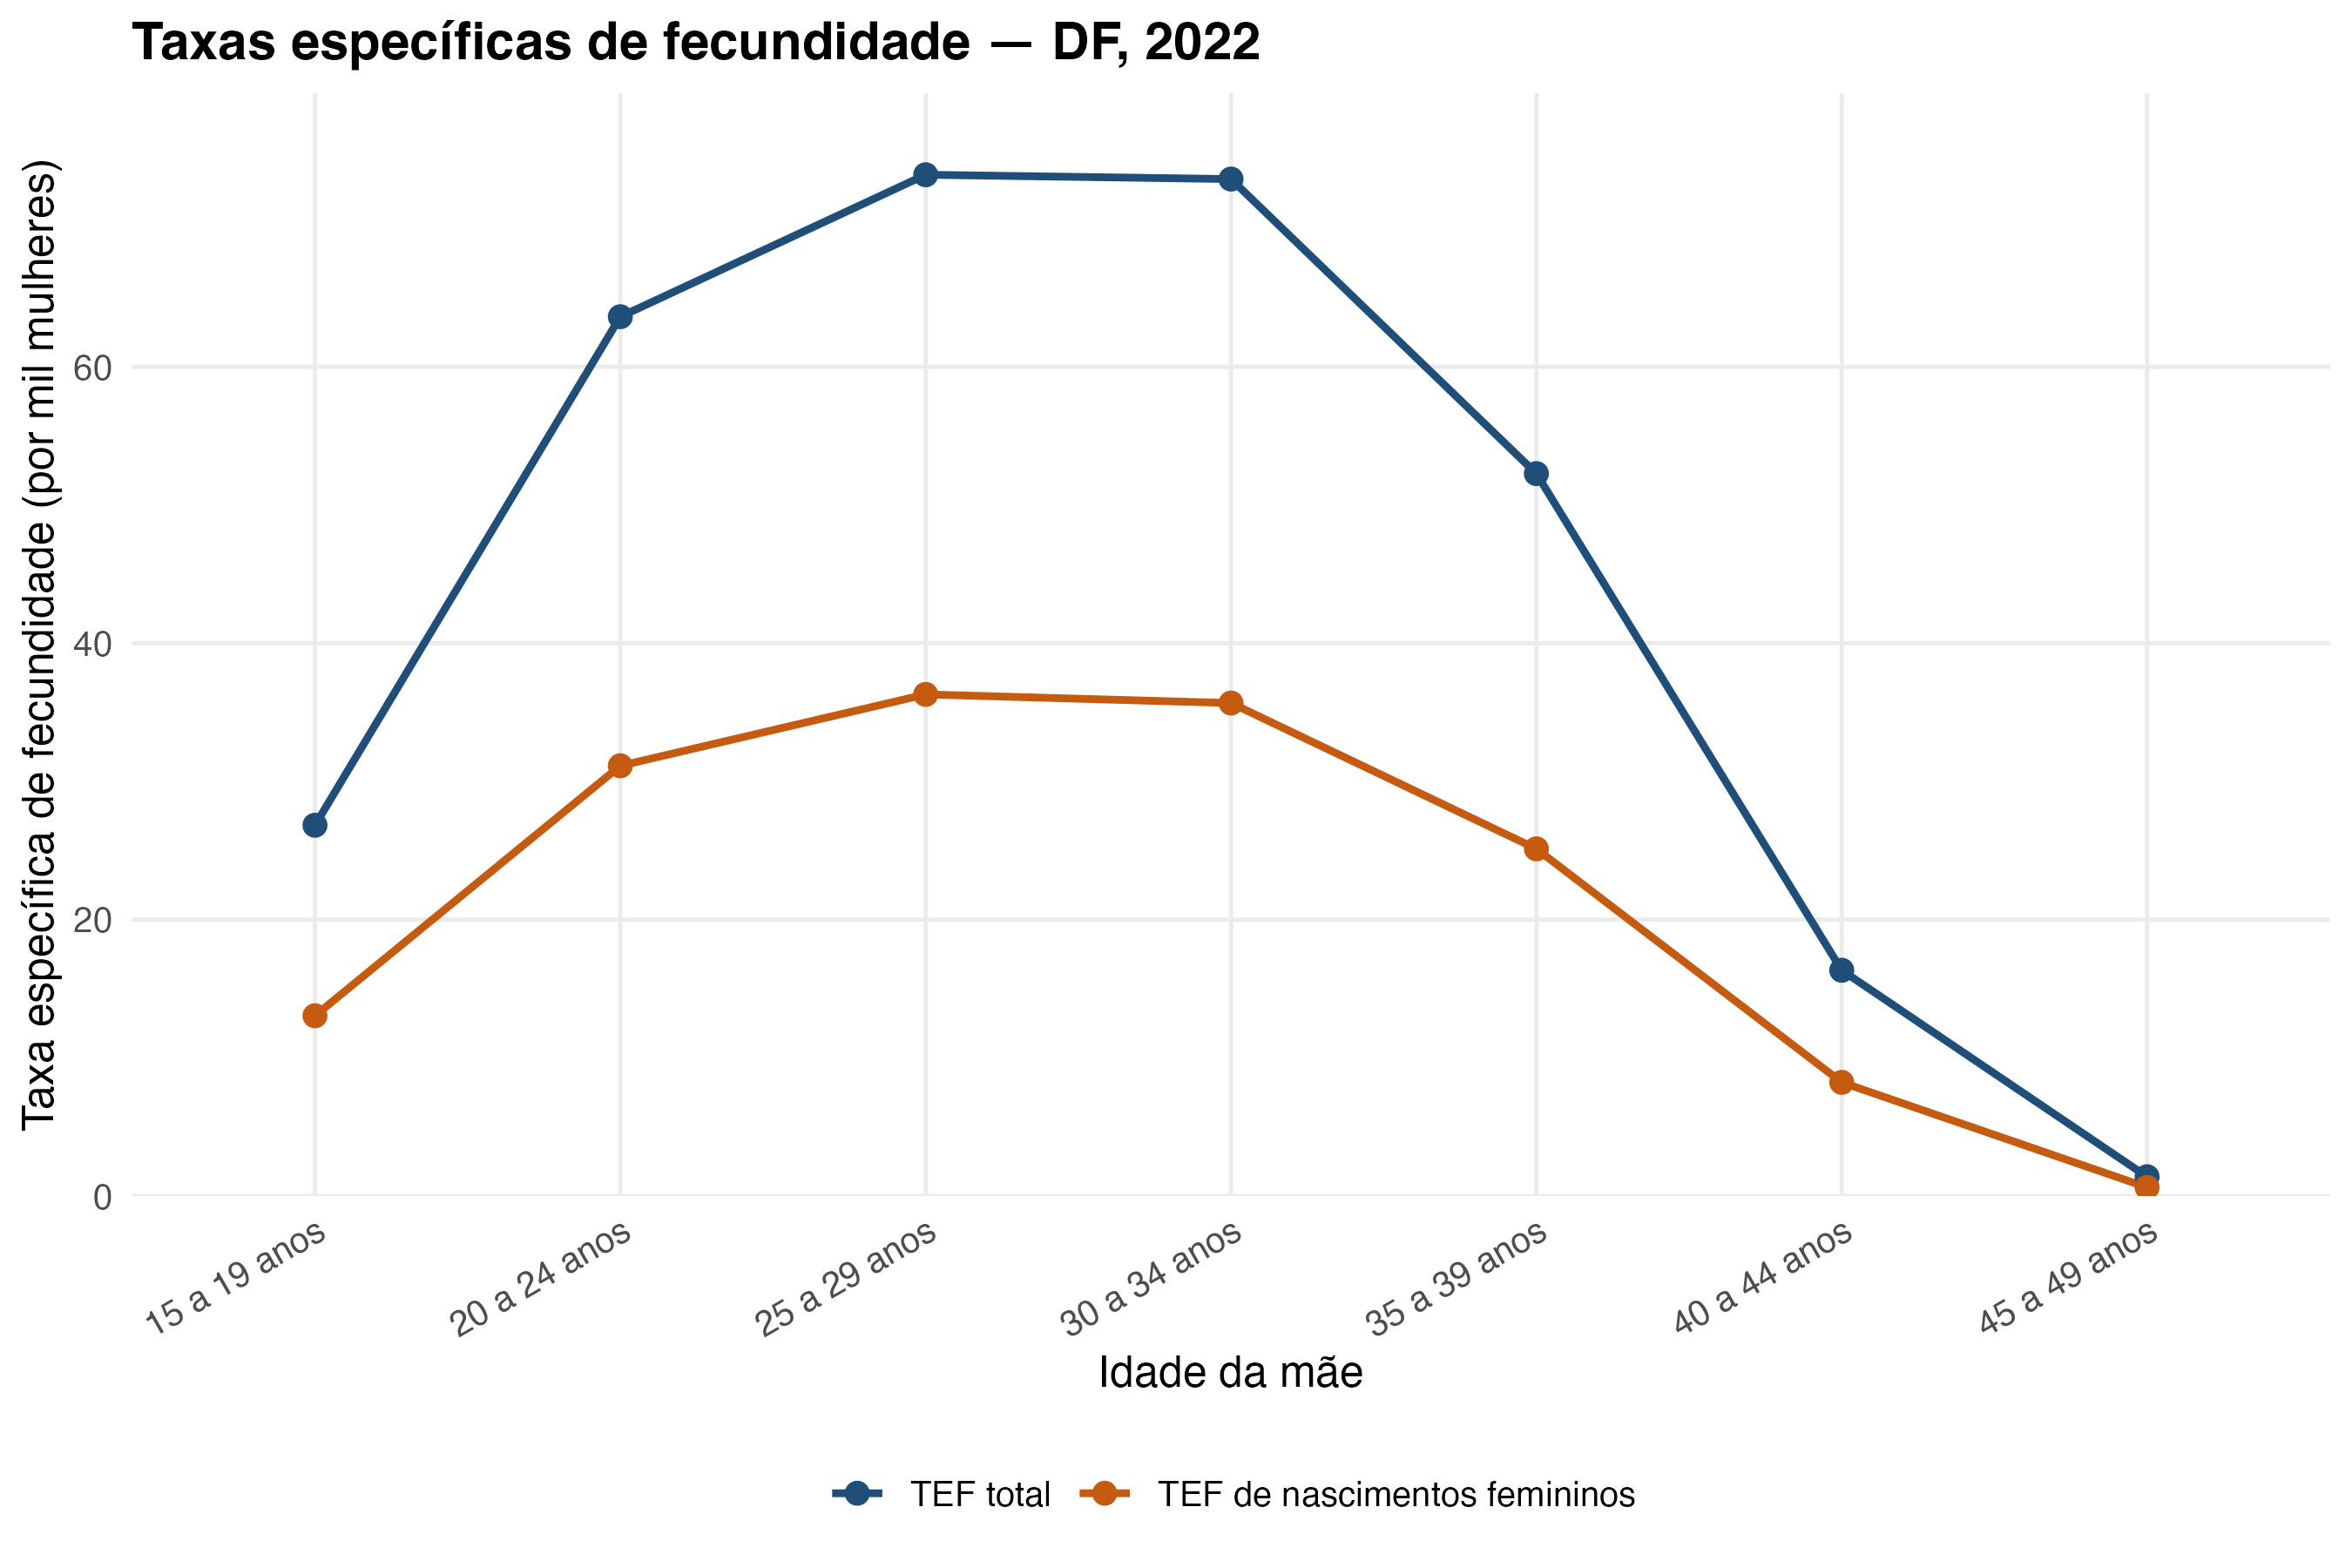
\includegraphics[width=0.88\textwidth]
{../figuras/grafico_item1_tef_df_2022.png}
\caption{Taxas específicas de fecundidade total e feminina, Distrito Federal, 2022}
\label{fig:tef_df_2022}
\fonte{Elaboração própria com dados do SINASC e do Censo Demográfico de 2022.}
\end{figure}

A distribuição apresentada na Figura~\ref{fig:tef_df_2022} indica concentração da fecundidade entre 20 e 39 anos, com máximo entre 25 e 29 anos e nível praticamente equivalente entre 30 e 34 anos. A proximidade entre esses dois grupos mostra que os nascimentos estavam distribuídos em um intervalo relativamente amplo das idades adultas. A curva referente às filhas mantém o mesmo formato da fecundidade total e apresenta níveis próximos da metade, conforme esperado pela distribuição dos nascimentos segundo o sexo.

\subsection{Idade média à maternidade}

A idade média à maternidade sintetiza a distribuição da fecundidade por idade e indica a idade média em que ocorreriam os nascimentos caso as taxas específicas observadas fossem mantidas. O indicador é calculado como uma média ponderada das idades centrais dos grupos etários, utilizando como pesos as respectivas contribuições para a fecundidade total \cite{grupofoz2021}:

\begin{equation}
\bar{m} =
\frac{\displaystyle\sum_{x=\alpha}^{\beta}\left(x+\frac{n}{2}\right)n\,{}_nf_x}
{\displaystyle\sum_{x=\alpha}^{\beta}n\,{}_nf_x},
\end{equation}

\noindent em que \(x+n/2\) é a idade central do grupo, \(n\) corresponde à amplitude do intervalo e \({}_nf_x\) representa a taxa específica de fecundidade total.

Para o Distrito Federal, a idade média à maternidade estimada foi de \textbf{29,37 anos}. Esse valor é consistente com o formato da curva de fecundidade, cujos níveis mais elevados se concentram nos grupos de 25 a 29 e de 30 a 34 anos. O resultado indica que o padrão reprodutivo de 2022 estava concentrado próximo dos 30 anos, com contribuição relevante das idades posteriores aos 30 para o nível total de fecundidade.

\subsection{Taxas bruta e líquida de reprodução}

A Taxa Bruta de Reprodução (TBR) representa o número médio de filhas que uma mulher teria ao longo do período reprodutivo caso fosse submetida às taxas de fecundidade feminina observadas, sem considerar a possibilidade de morte antes do término desse período. Para grupos etários de amplitude \(n\), o indicador foi calculado por \cite{grupofoz2021,preston2001}:

\begin{equation}
TBR = \sum_{x=\alpha}^{\beta} n\,{}_nf_x^F,
\end{equation}

\noindent em que \({}_nf_x^F\) corresponde à taxa específica de fecundidade referente ao nascimento de filhas no grupo etário iniciado em \(x\).

A Taxa Líquida de Reprodução (TLR) incorpora a sobrevivência feminina desde o nascimento até as idades reprodutivas. Para cada grupo, a fecundidade feminina foi ponderada pela proporção média sobrevivente, obtida a partir da tábua de vida:

\begin{equation}
TLR =
\sum_{x=\alpha}^{\beta}{}_nf_x^F
\frac{{}_nL_x^F}{\ell_0^F},
\end{equation}

\noindent em que \({}_nL_x^F\) representa os anos-pessoa vividos pelas mulheres no intervalo e \(\ell_0^F\) é a raiz da tábua de vida feminina. Como \({}_nL_x^F\) já incorpora a amplitude do intervalo, não se acrescenta outro fator \(n\) à soma.

\begin{table}[H]
    \centering
    \caption{Taxas de reprodução, Distrito Federal, 2022}
    \label{tab:tbr_tlr}
    \begin{tabular}{lc}
        \toprule
        Indicador & Filhas por mulher \\
        \midrule
        Taxa Bruta de Reprodução (TBR)   & 0,7506 \\
        Taxa Líquida de Reprodução (TLR) & 0,7336 \\
        \bottomrule
    \end{tabular}
    
    \vspace{0.2cm}
    \fonte{Elaboração própria com dados do SINASC, SIM e Censo Demográfico de 2022.}
\end{table}

Os dois indicadores ficaram abaixo de uma filha por mulher, nível necessário para a reposição de 
uma geração feminina por outra. A TLR de 0,7336 indica que, mantidas as condições de fecundidade 
e mortalidade de 2022, cada geração de mulheres seria substituída por outra aproximadamente 
26,64\% menor, na ausência de migração. A pequena diferença entre TBR e TLR mostra que a mortalidade anterior e durante as idades reprodutivas reduz a reprodução potencial, mas seu efeito é relativamente limitado quando comparado ao baixo nível da fecundidade.


\section{Taxa intrínseca de crescimento}

A taxa intrínseca de crescimento, \(r\), corresponde à taxa constante de variação de uma população estável submetida indefinidamente a determinadas funções de fecundidade e mortalidade, na ausência de migração. Diferentemente da taxa de crescimento observada, seu valor elimina o efeito da estrutura etária corrente e representa o potencial de crescimento associado às condições demográficas analisadas \cite{grupofoz2021,preston2001}.

\subsection{Aproximação pela taxa líquida de reprodução}

Uma aproximação de \(r\) pode ser obtida relacionando a TLR à idade média da função líquida de maternidade:

\begin{equation}
r_0 \approx \frac{\ln(TLR)}{T_0},
\end{equation}

\noindent em que
\begin{equation}
T_0=\frac{\displaystyle\sum_{x=\alpha}^{\beta}
\left(x+\frac{n}{2}\right){}_nf_x^F
\dfrac{{}_nL_x^F}{\ell_0^F}}{TLR}.
\end{equation}
Para o Distrito Federal, obteve-se \(T_0=29,33\) anos. Com \(TLR=0,7336\), a aproximação resultou em \(r_0=-0,0105622\) ao ano. Os valores \(-1,0562\%\) e \(-10,5622\) por mil apresentados adiante correspondem, respectivamente, a \(100r_0\) e \(1.000r_0\).

\subsection{Equação de Euler--Lotka}

A estimativa mais precisa foi obtida pela solução numérica da forma discreta da equação de Euler--Lotka:

\begin{equation}
\sum_{x=\alpha}^{\beta}
e^{-r\left(x+n/2\right)}
{}_nf_x^F
\frac{{}_nL_x^F}{\ell_0^F}=1,
\end{equation}

\noindent em que \(x+n/2\) é a idade central do grupo e os demais termos correspondem à contribuição líquida da fecundidade feminina. A raiz da equação foi determinada numericamente no R.

\begin{table}[H]
\centering
\caption{Taxa intrínseca de crescimento segundo o método de estimação}
\label{tab:r_intrinseco}
\begin{tabular}{lrr}
\toprule
Método & $100r$ (\% ao ano) & $1.000r$ (por mil ao ano) \\  
\midrule
Aproximação pela TLR & $-1,0562$ & $-10,5622$ \\
Equação de Lotka     & $-1,0474$ & $-10,4741$ \\
\bottomrule
\end{tabular}


\vspace{0.2cm}
\fonte{Elaboração própria com dados do SINASC, SIM e Censo Demográfico de 2022.}


\end{table}

Os dois procedimentos produziram resultados muito próximos, com diferença de apenas 0,0881 por 
mil ao ano na escala \(1.000r\). A solução da equação de Euler--Lotka, \(r=-0,0104741\), foi adotada nos cálculos 
subsequentes. O sinal negativo indica que as condições de fecundidade e mortalidade de 2022 
implicariam redução anual de aproximadamente 1,05\% em uma população estável e fechada. 
Esse resultado não corresponde necessariamente à variação populacional efetivamente observada 
no Distrito Federal, pois esta também é influenciada pela migração e pela estrutura etária 
existente.


\section{População estável intrínseca}

Uma população estável é produzida pela manutenção de funções de fecundidade e mortalidade constantes ao longo do tempo, sob a hipótese de ausência de migração. Depois de transcorrido o período de convergência, sua distribuição relativa por idade permanece constante, enquanto o tamanho populacional varia exponencialmente à taxa intrínseca \(r\). A taxa de crescimento, a estrutura etária e as taxas brutas dessa população são determinadas exclusivamente pelas funções de fecundidade e sobrevivência adotadas \cite{grupofoz2021,preston2001}.

\subsection{Taxa bruta de natalidade}

A taxa bruta de natalidade da população estável expressa o número anual de nascimentos por unidade de população na estrutura etária correspondente ao valor intrínseco de \(r\). Para incluir ambos os sexos, foram consideradas as proporções masculina e feminina observadas entre os nascimentos e as funções de sobrevivência das respectivas tábuas de vida. O cálculo foi realizado por:

\begin{equation}
TBN =
\left[
\sum_s p_s
\sum_{x=0}^{\omega}
e^{-r a_x}
\frac{{}_nL_x^s}{\ell_0^s}
\right]^{-1},
\end{equation}

\noindent em que \(p_s\) representa a proporção de nascimentos do sexo \(s\), \(a_x=x+n/2\) é a idade representativa dos intervalos fechados, \({}_nL_x^s\) corresponde aos anos-pessoa vividos e \(\ell_0^s\) é a raiz da respectiva tábua de vida. Para o intervalo aberto de 80 anos ou mais, adotou-se \(a_{80}=80+e_{80}^s\).

A taxa estimada foi \(TBN=0,00779804\) ao ano, equivalente a \textbf{7,798 nascimentos por mil habitantes}. O valor é inferior à taxa intrínseca de mortalidade implícita, pois a relação \(r=TBN-TBM\), combinada ao valor negativo de \(r\), exige que os óbitos superem os nascimentos na população estável. Portanto, mantidas as condições demográficas de 2022 e desconsiderada a migração, a estrutura estável equivalente seria compatível com redução populacional.

\subsection{Estrutura etária pelo método de Lotka}

No modelo de Lotka, a participação relativa de cada grupo etário na população estável depende da sobrevivência até a idade considerada e do crescimento acumulado entre o nascimento da coorte e o momento de referência. Para cada sexo, foram calculados pesos proporcionais a:

\begin{equation}
{}_nP_x^s
\propto
p_s e^{-r a_x}
\frac{{}_nL_x^s}{\ell_0^s},
\end{equation}

\noindent em que \(p_s\) é a proporção de nascimentos do sexo \(s\), \(r\) é a taxa intrínseca 
obtida pela equação de Euler--Lotka e \(a_x\) corresponde à idade representativa do intervalo. 
Os pesos masculinos e femininos foram normalizados conjuntamente, de modo que a soma da 
estrutura resultasse em 100\% \cite{grupofoz2021,preston2001}.

\begin{figure}[H]
\centering
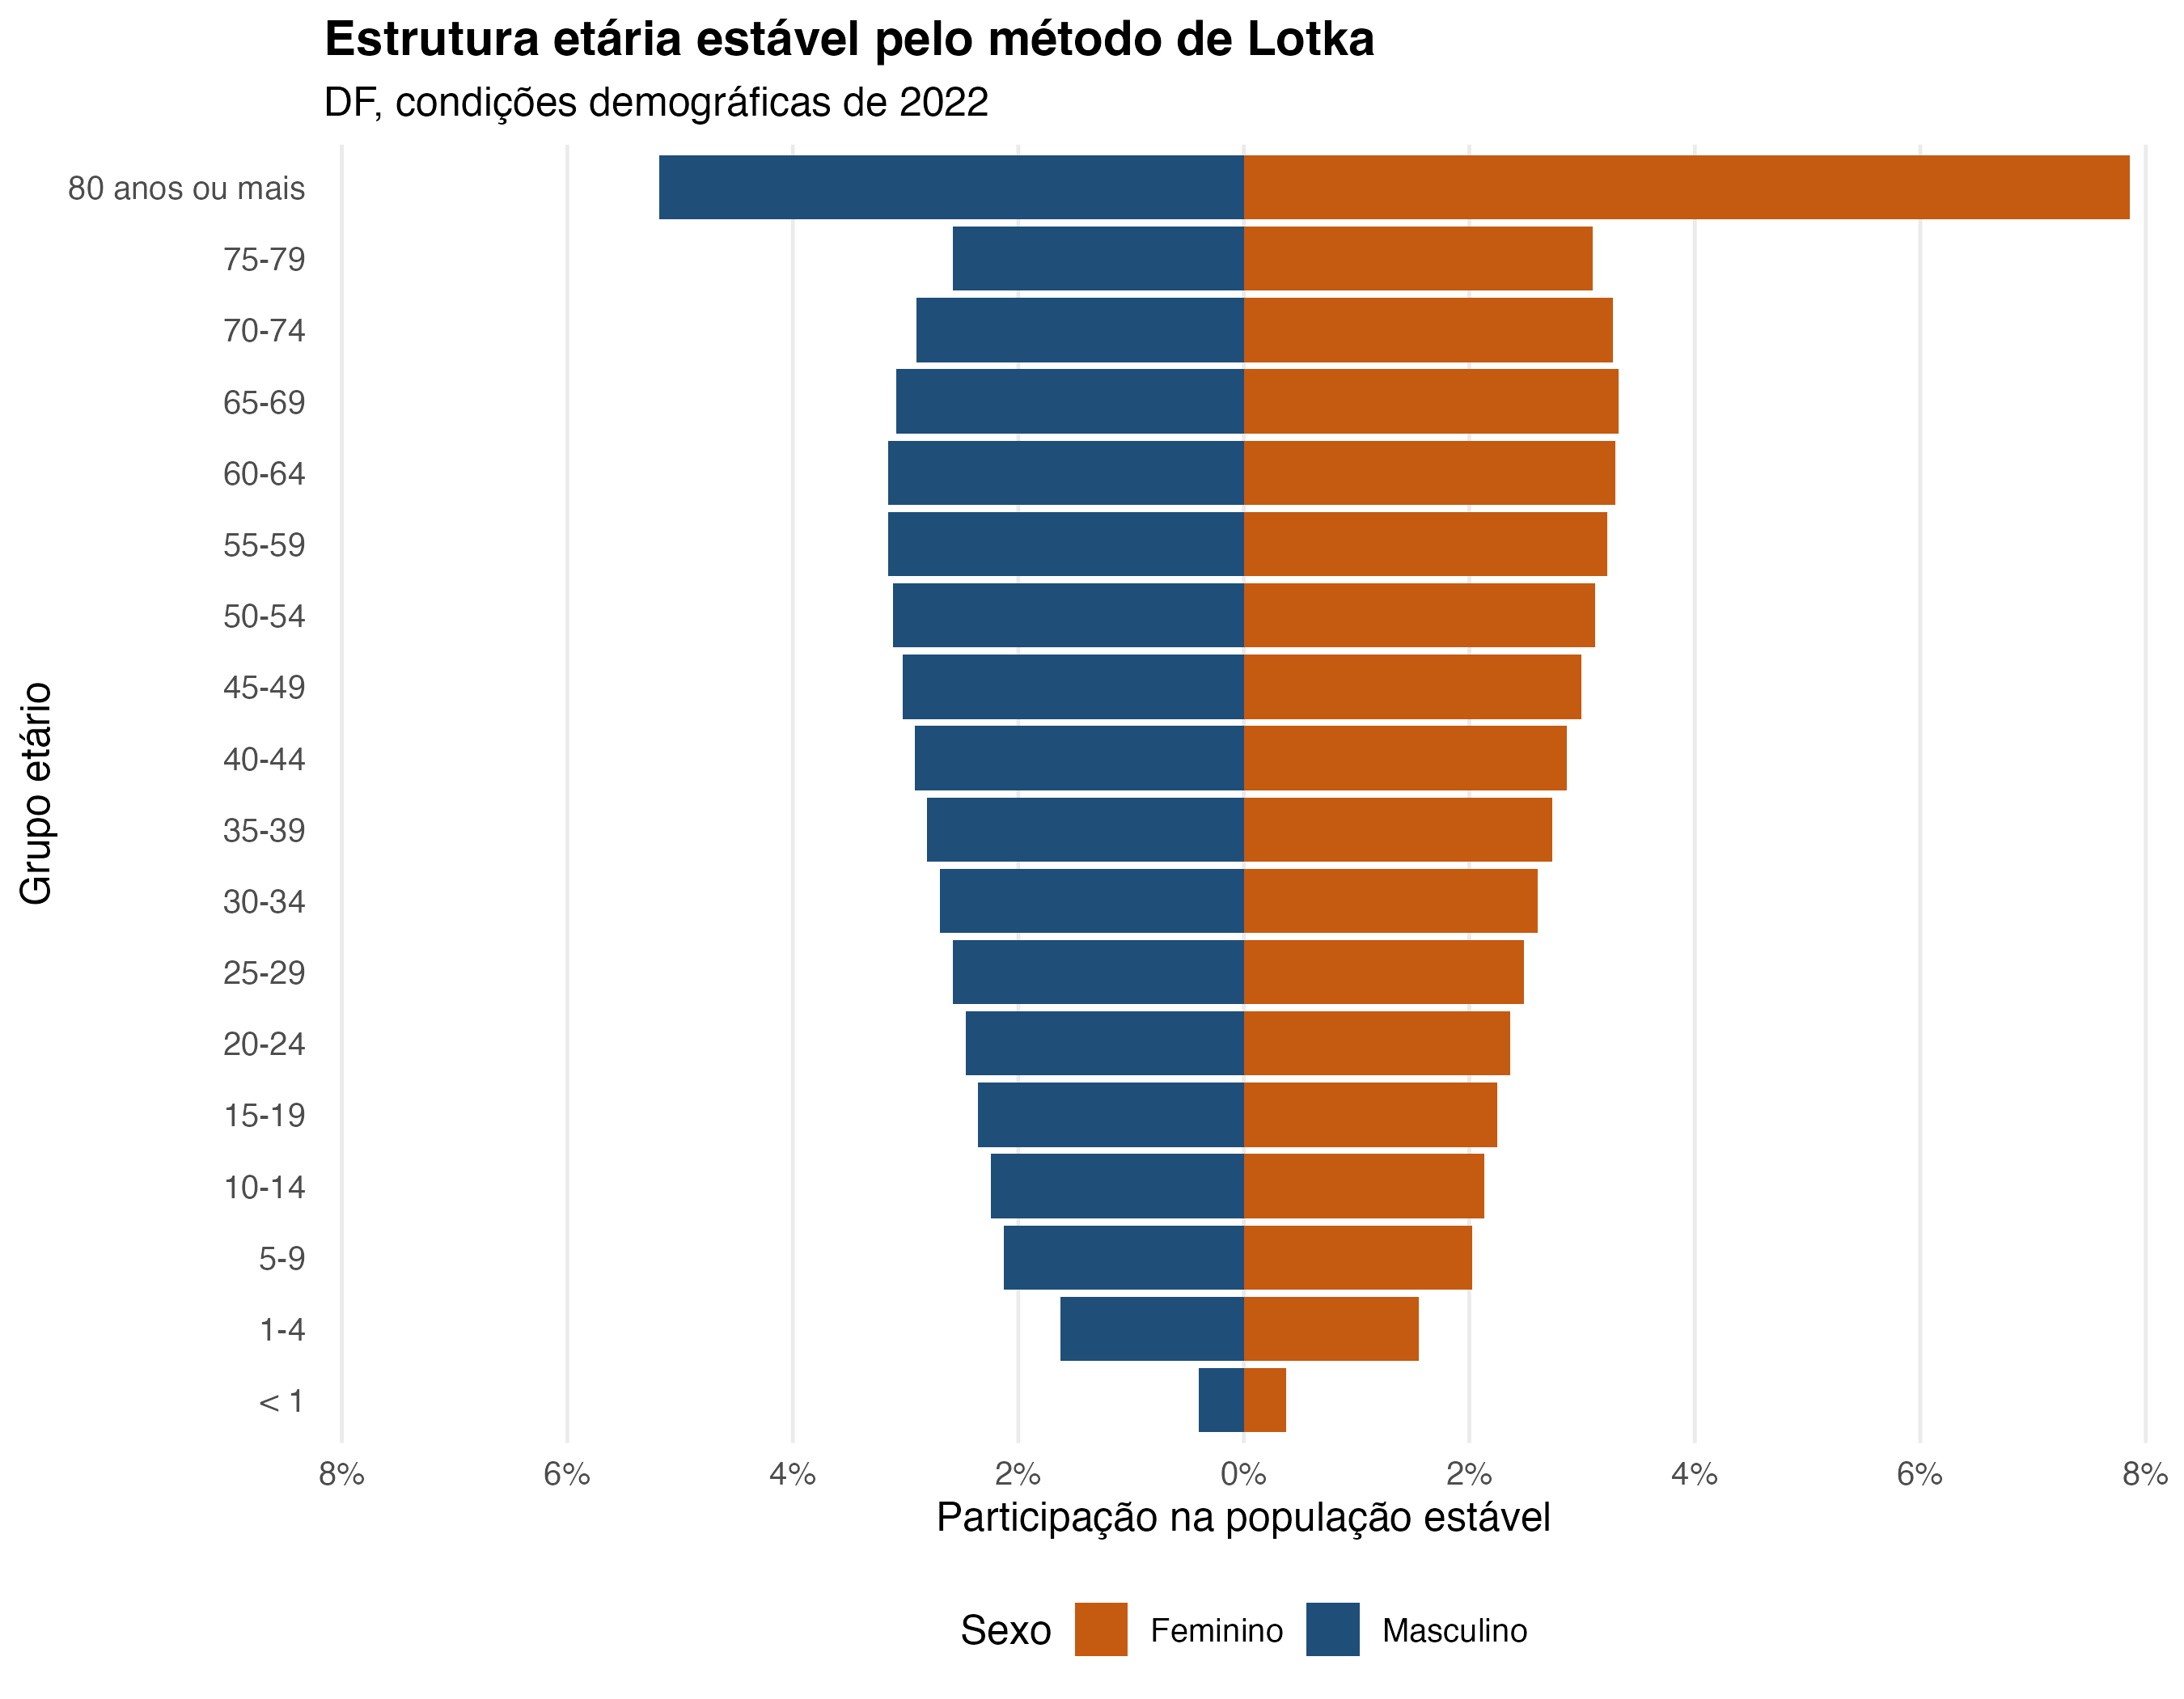
\includegraphics[width=0.85\textwidth]
{../figuras/piramide_estrutura_estavel_lotka_df_2022.png}
\caption{Estrutura etária estável pelo método de Lotka, Distrito Federal, 2022}
\label{fig:estrutura_lotka}
\fonte{Elaboração própria com dados do SINASC, SIM e Censo Demográfico de 2022.}
\end{figure}

A estrutura obtida apresenta base estreita e elevada participação das idades avançadas, 
resultado compatível com a taxa intrínseca negativa. Na distribuição total, 12,49\% da população 
estaria entre 0 e 14 anos, 56,21\% entre 15 e 64 anos e 31,30\% teria 65 anos ou mais. 
A participação feminina torna-se superior nas idades mais elevadas em razão de sua maior 
sobrevivência. O grupo aberto de 80 anos ou mais concentra todas as idades posteriores e, 
por isso, não deve ser comparado diretamente a um único grupo quinquenal.

\subsection{Estrutura etária pelo método matricial de Leslie}

A matriz de Leslie representa a dinâmica populacional em tempo discreto, combinando fecundidade e sobrevivência por idade. Neste trabalho, utilizou-se um intervalo de projeção de cinco anos e 17 grupos etários, de 0--4 anos até 80 anos ou mais. A evolução da população é dada por

\begin{equation}
    \mathbf{P}(t+n) = \mathbf{L}\mathbf{P}(t), \qquad n=5.
\end{equation}

\noindent em que $\mathbf{P}(t)$ é o vetor populacional no instante $t$ e $\mathbf{L}$ é a matriz de projeção. Na implementação adotou-se uma versão simplificada: os elementos de fecundidade foram obtidos de \(n\,{}_nf_x^F\), e as probabilidades de sobrevivência entre idades exatas, de \(S_x^s=\ell_{x+n}^s/\ell_x^s\). No intervalo aberto de 80 anos ou mais, também foi incorporada a permanência dos sobreviventes no próprio grupo \cite{grupofoz2021,preston2001}.

Inicialmente, construiu-se a matriz para a população feminina, utilizando as taxas específicas de fecundidade de nascimentos femininos e as relações de sobrevivência obtidas da tábua de vida feminina. Em seguida, a formulação foi ampliada para os dois sexos, com a distribuição dos nascimentos segundo a proporção observada de nascidos vivos femininos e masculinos e com funções de sobrevivência específicas por sexo.

A estrutura etária estável corresponde ao autovetor associado ao autovalor dominante da matriz:

\begin{equation}
\mathbf{L}\mathbf{w}=\lambda\mathbf{w},
\end{equation}

\noindent em que $\lambda$ representa o fator de crescimento em cada intervalo quinquenal e $\mathbf{w}$ representa a estrutura etária estável. A relação entre o autovalor e a taxa contínua é \(\lambda=e^{rn}\), ou \(r=\ln(\lambda)/n\). O autovetor foi normalizado de forma que a soma de seus componentes, considerando ambos os sexos, fosse igual a um \cite{grupofoz2021,preston2001}.

Na estrutura estimada, a população de 0 a 14 anos corresponde a 12,40\% do total, a população 
de 15 a 64 anos representa 54,46\% e o grupo de 65 anos ou mais alcança 33,14\%. A composição 
por sexo resultou em 51,45\% de mulheres e 48,55\% de homens. A maior participação feminina nas 
idades avançadas decorre da menor mortalidade feminina observada nas tábuas de vida.

A estrutura obtida apresenta base relativamente estreita e elevada concentração nas idades 
mais avançadas. Esse formato decorre da combinação entre fecundidade inferior ao nível de 
reposição e maior sobrevivência até idades elevadas. Assim, se as condições demográficas de 
2022 permanecessem constantes e não houvesse migração, a população convergiria para uma 
estrutura consideravelmente mais envelhecida que a observada no Censo de 2022.

\begin{figure}[H]
\centering
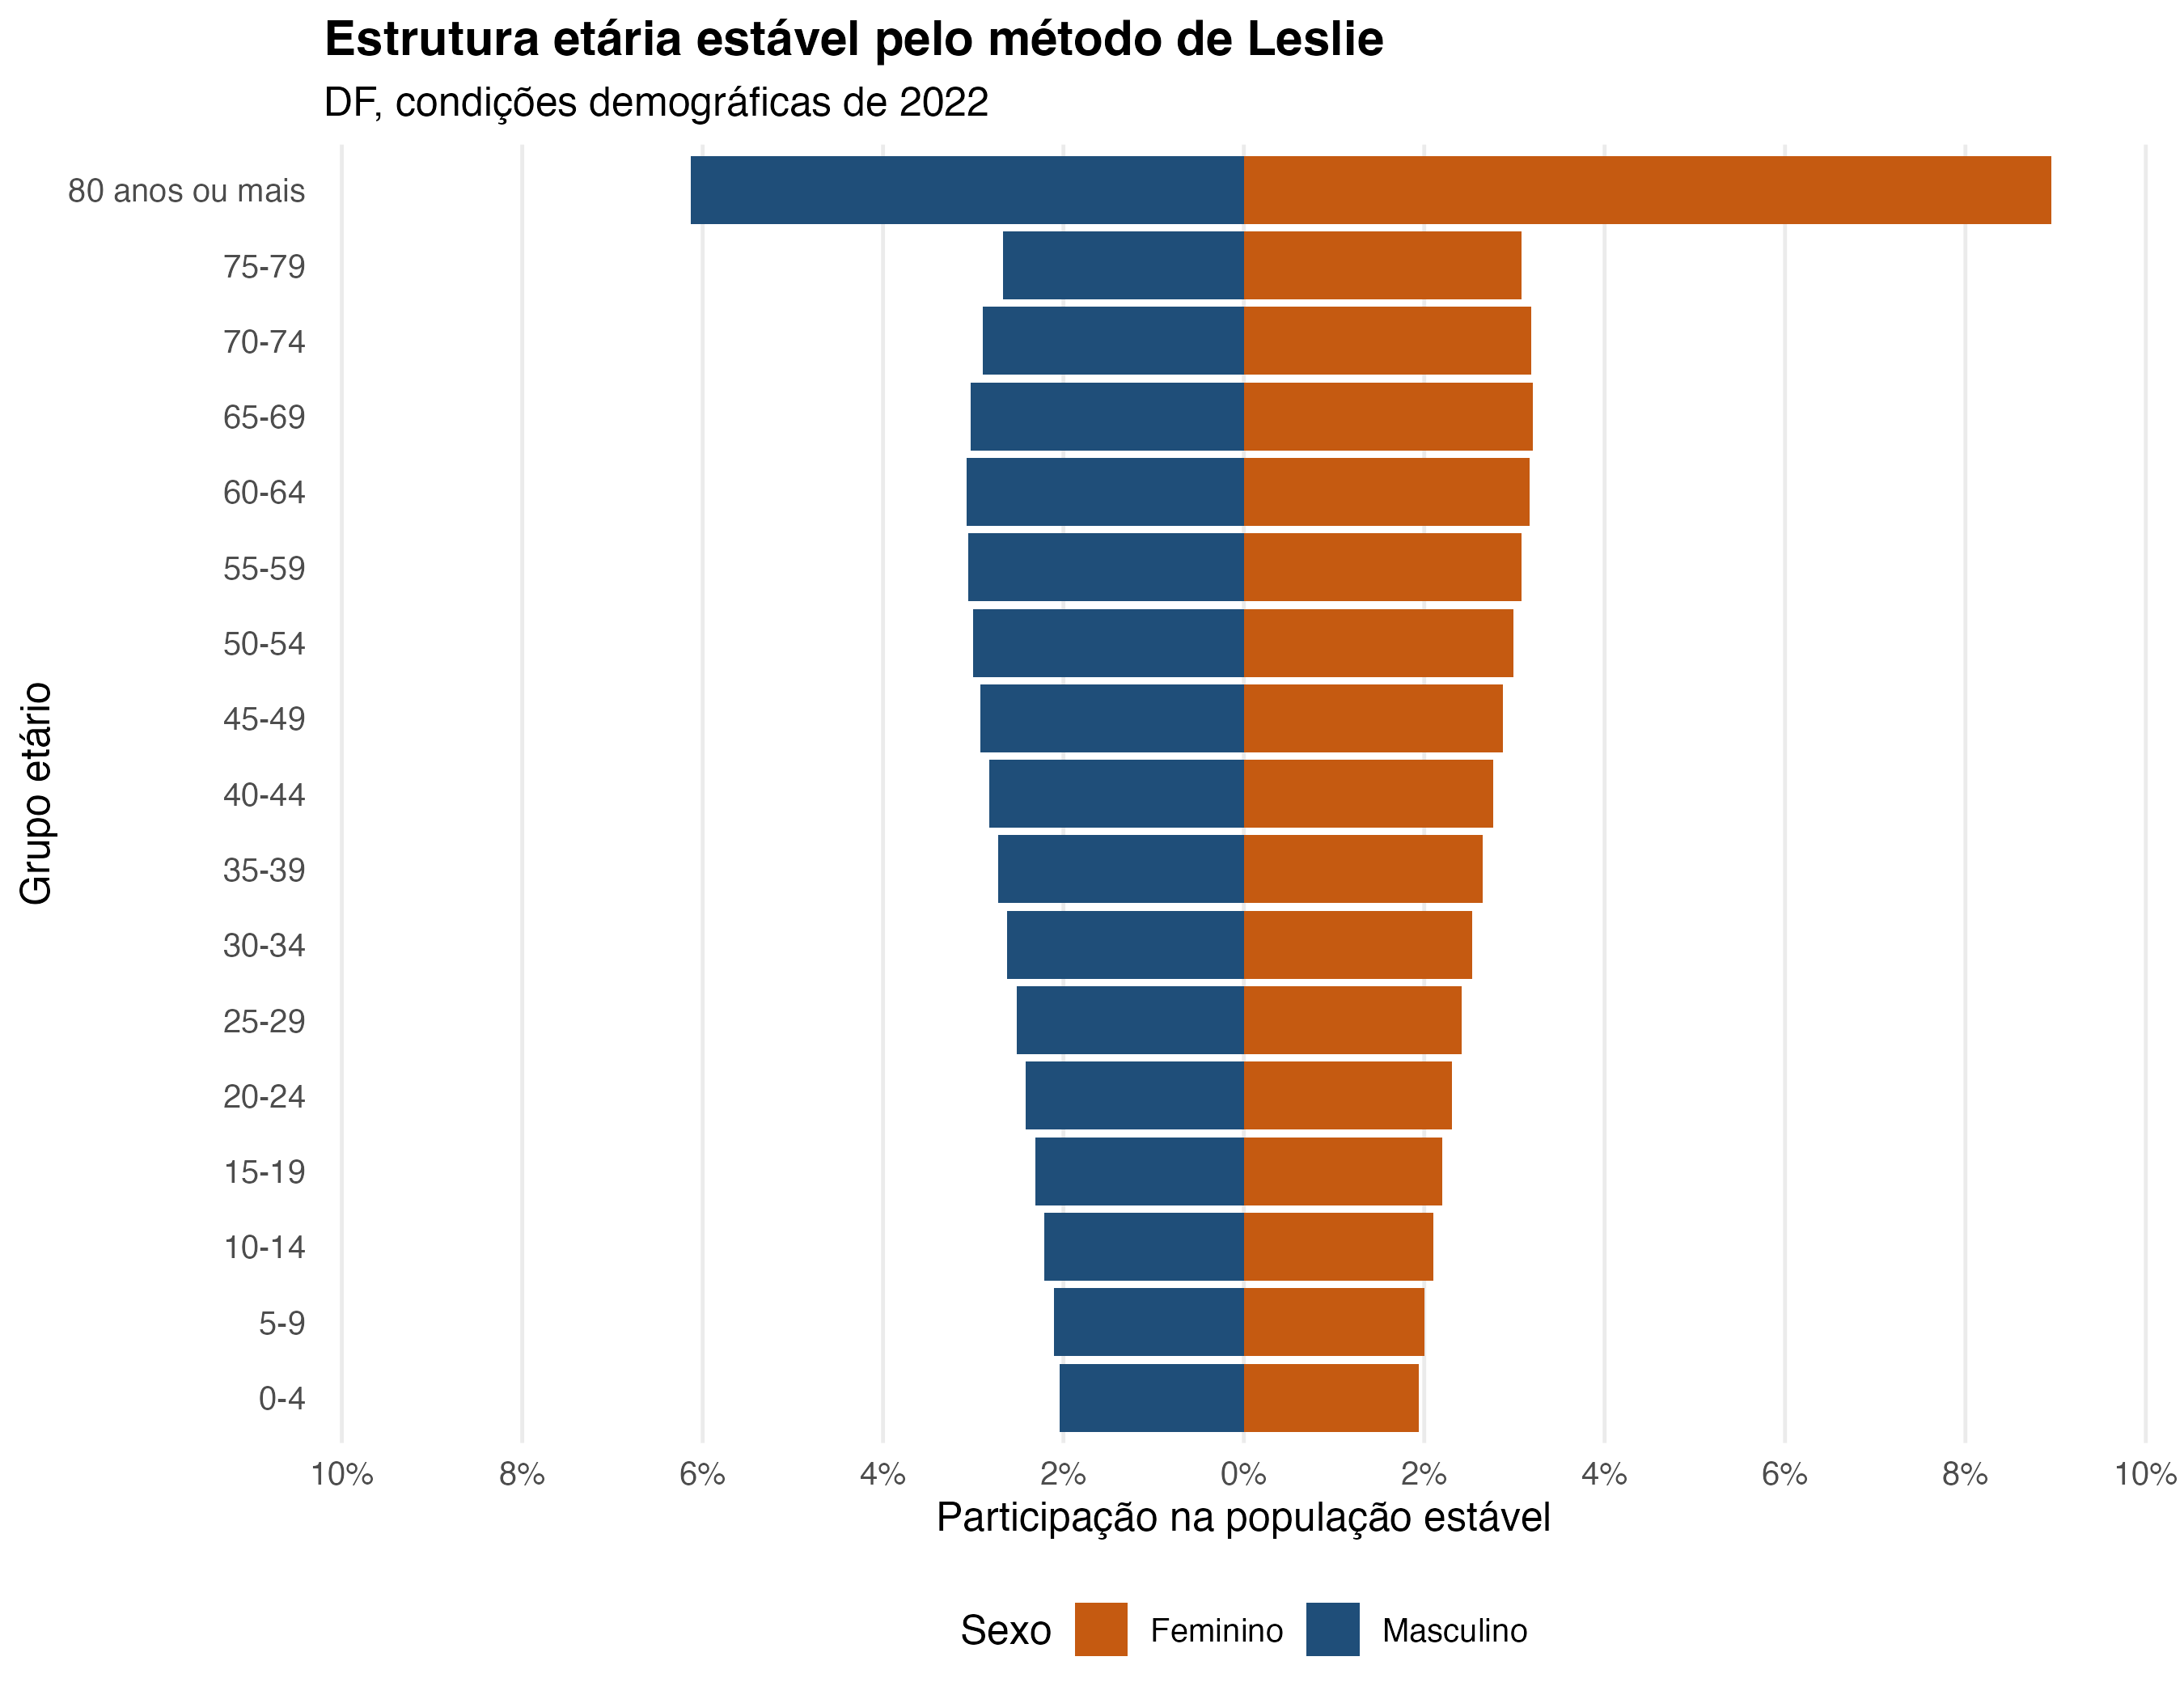
\includegraphics[width=0.92\textwidth]
{../figuras/piramide_estrutura_estavel_leslie_df_2022.png}
\caption{Estrutura etária estável estimada pelo método matricial de Leslie, Distrito Federal, 2022}
\label{fig:estrutura_leslie}
\fonte{Elaboração própria com dados do SINASC, SIM e Censo Demográfico de 2022.}
\end{figure}


\section{Comparação com a estrutura etária observada}

A estrutura etária observada foi calculada a partir da população recenseada do Distrito Federal em 2022, agrupada em intervalos quinquenais de idade e por sexo. Diferentemente das estruturas de Lotka e Leslie, a distribuição observada incorpora os efeitos acumulados das variações históricas da fecundidade, da mortalidade e, especialmente, da migração.

\begin{figure}[H]
\centering
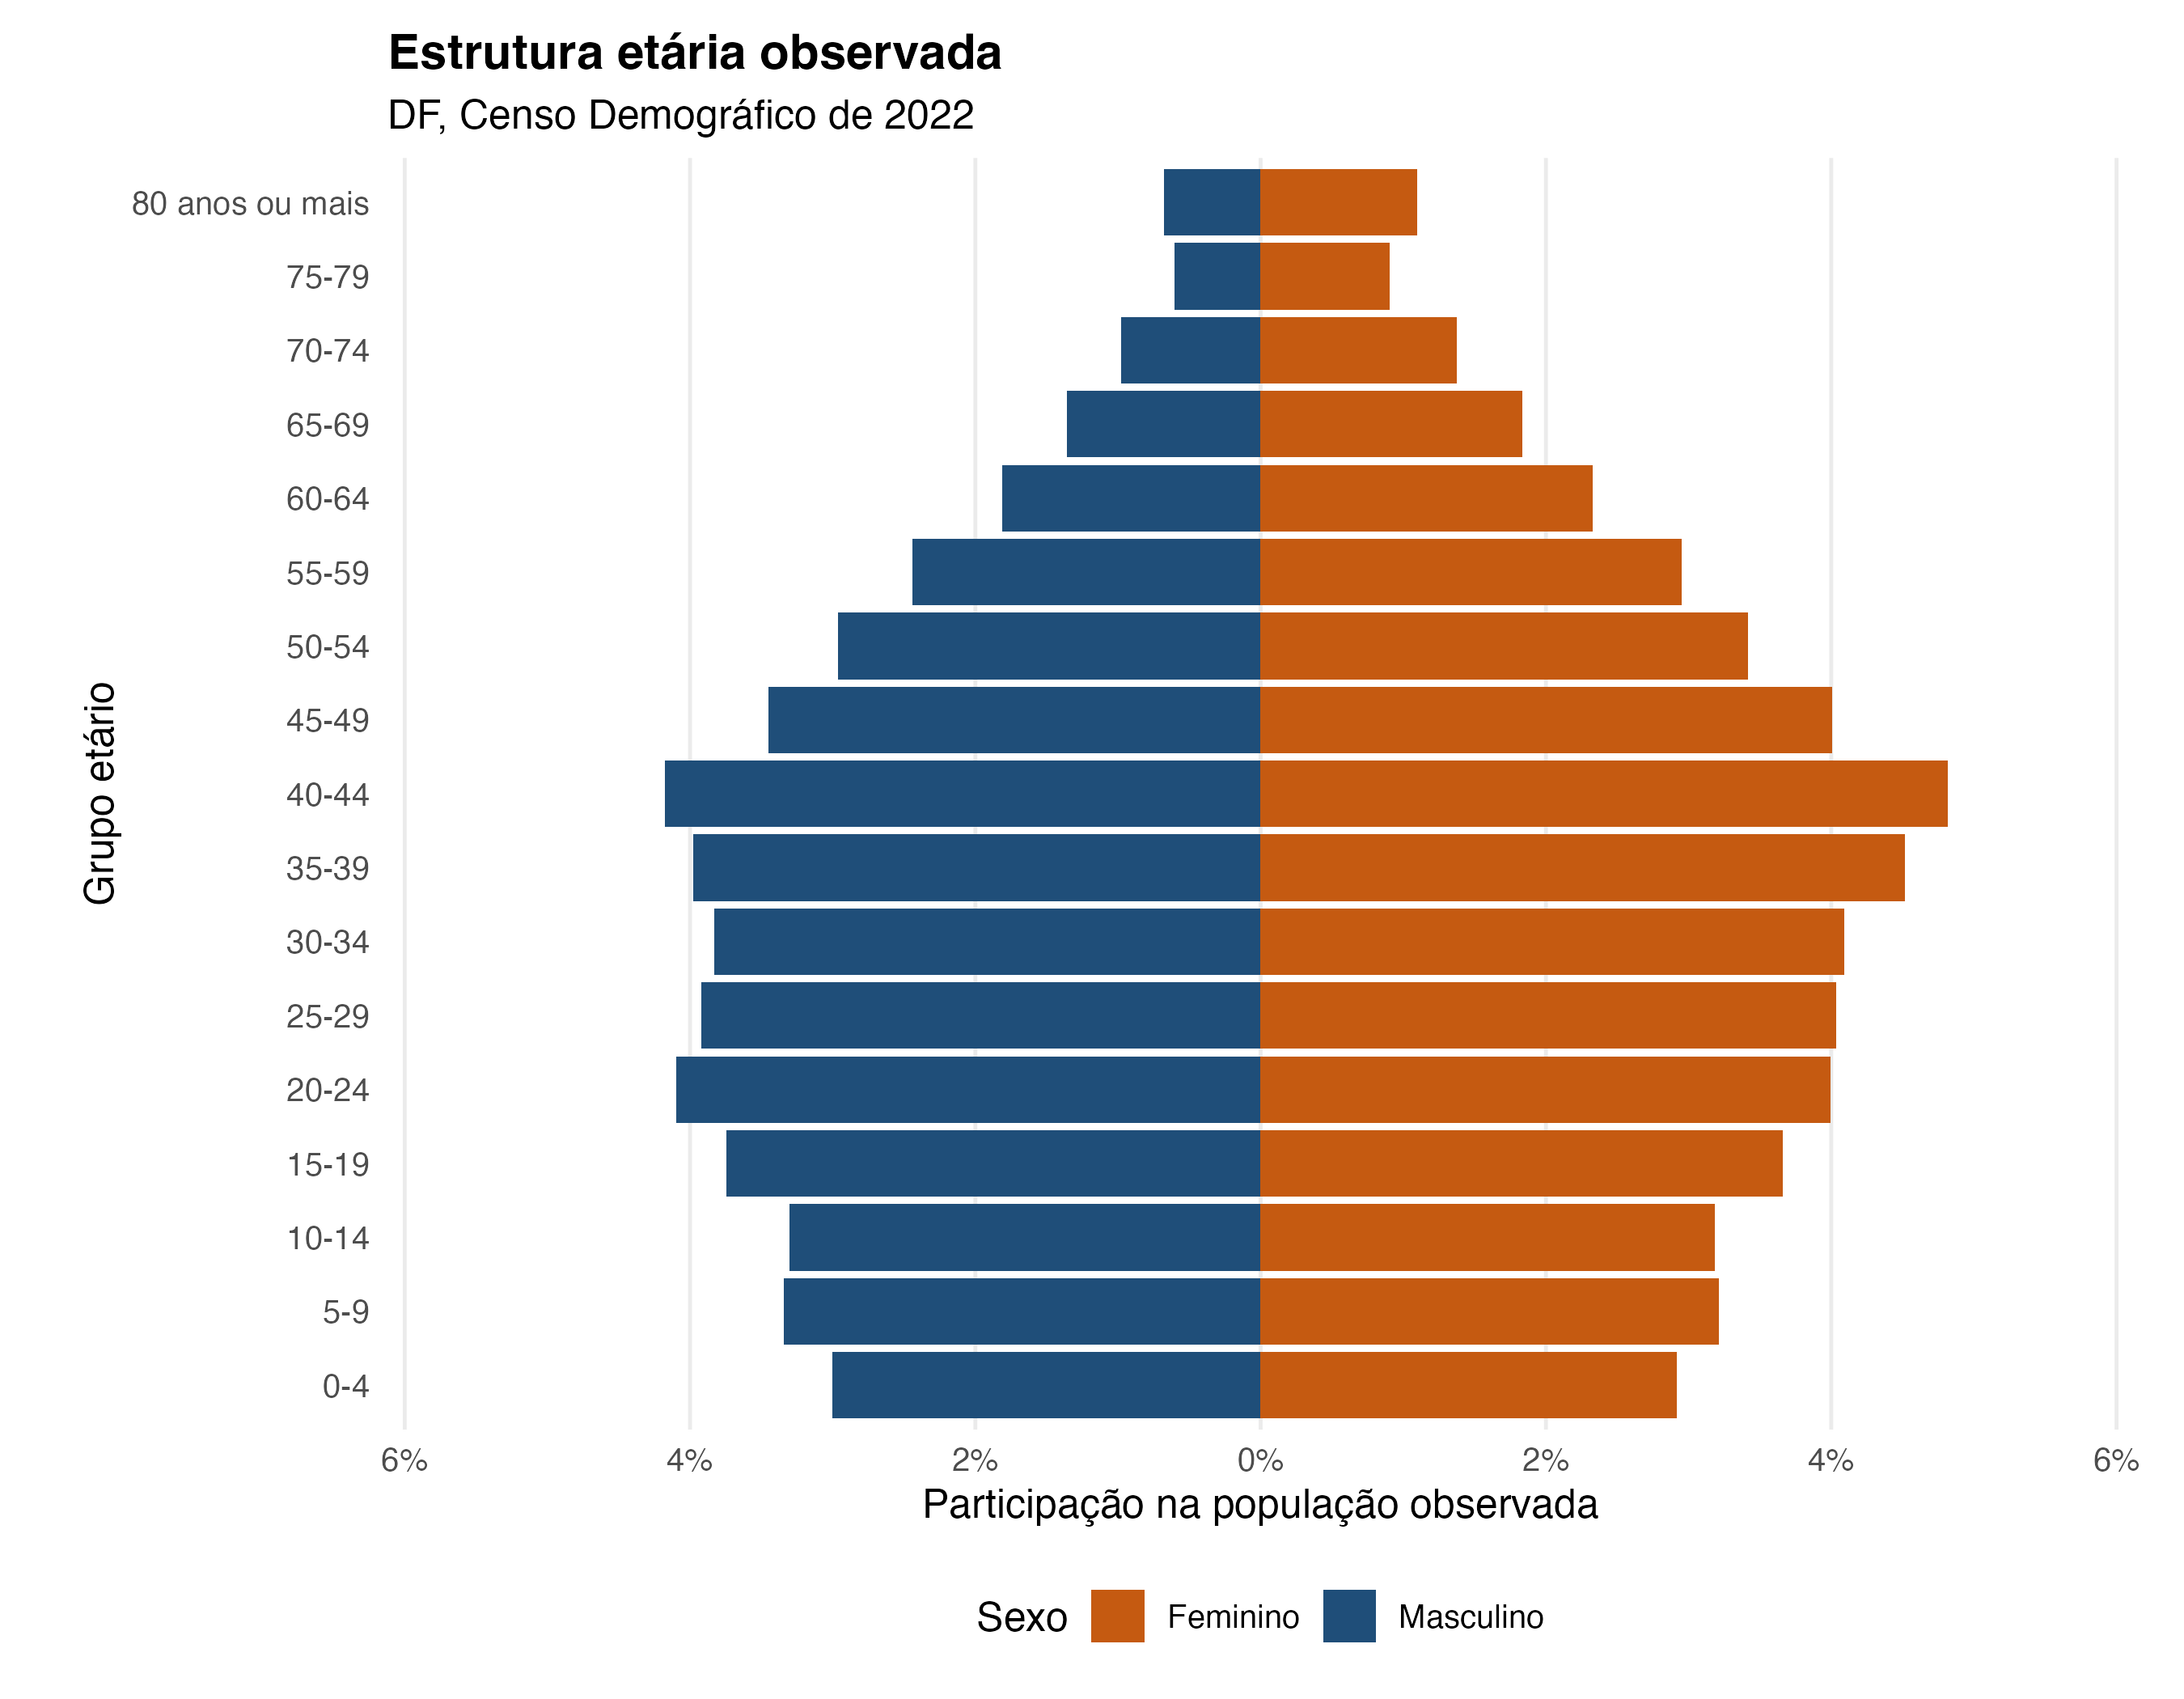
\includegraphics[width=0.90\textwidth]
{../figuras/piramide_estrutura_observada_df_2022.png}
\caption{Estrutura etária observada, Distrito Federal, 2022}
\label{fig:estrutura_observada}
\vspace{0.2cm}
\fonte{Elaboração própria com dados do Censo Demográfico de 2022.}
\end{figure}

A estrutura observada apresenta maior concentração nas idades adultas, principalmente entre 20 e 49 anos, e participação relativamente reduzida nas idades mais avançadas. Esse formato reflete tanto a redução recente da fecundidade quanto a atração migratória exercida pelo Distrito Federal sobre indivíduos em idade economicamente ativa.

\begin{table}[H]
\centering
\caption{Distribuição da população por grandes grupos etários, segundo a estrutura considerada}
\label{tab:comparacao_grupos}
\begin{tabular}{lccc}
\toprule
\textbf{Estrutura} & \textbf{0 a 14 anos} &
\textbf{15 a 64 anos} & \textbf{65 anos ou mais} \\
\midrule
Observada & 18,96\% & 72,22\% & 8,82\% \\
Lotka     & 12,49\% & 56,21\% & 31,30\% \\
Leslie    & 12,40\% & 54,46\% & 33,14\% \\
\bottomrule
\end{tabular}


\vspace{0.2cm}
\fonte{Elaboração própria com dados do Censo Demográfico, SINASC e SIM de 2022.}


\end{table}

\begin{figure}[H]
\centering
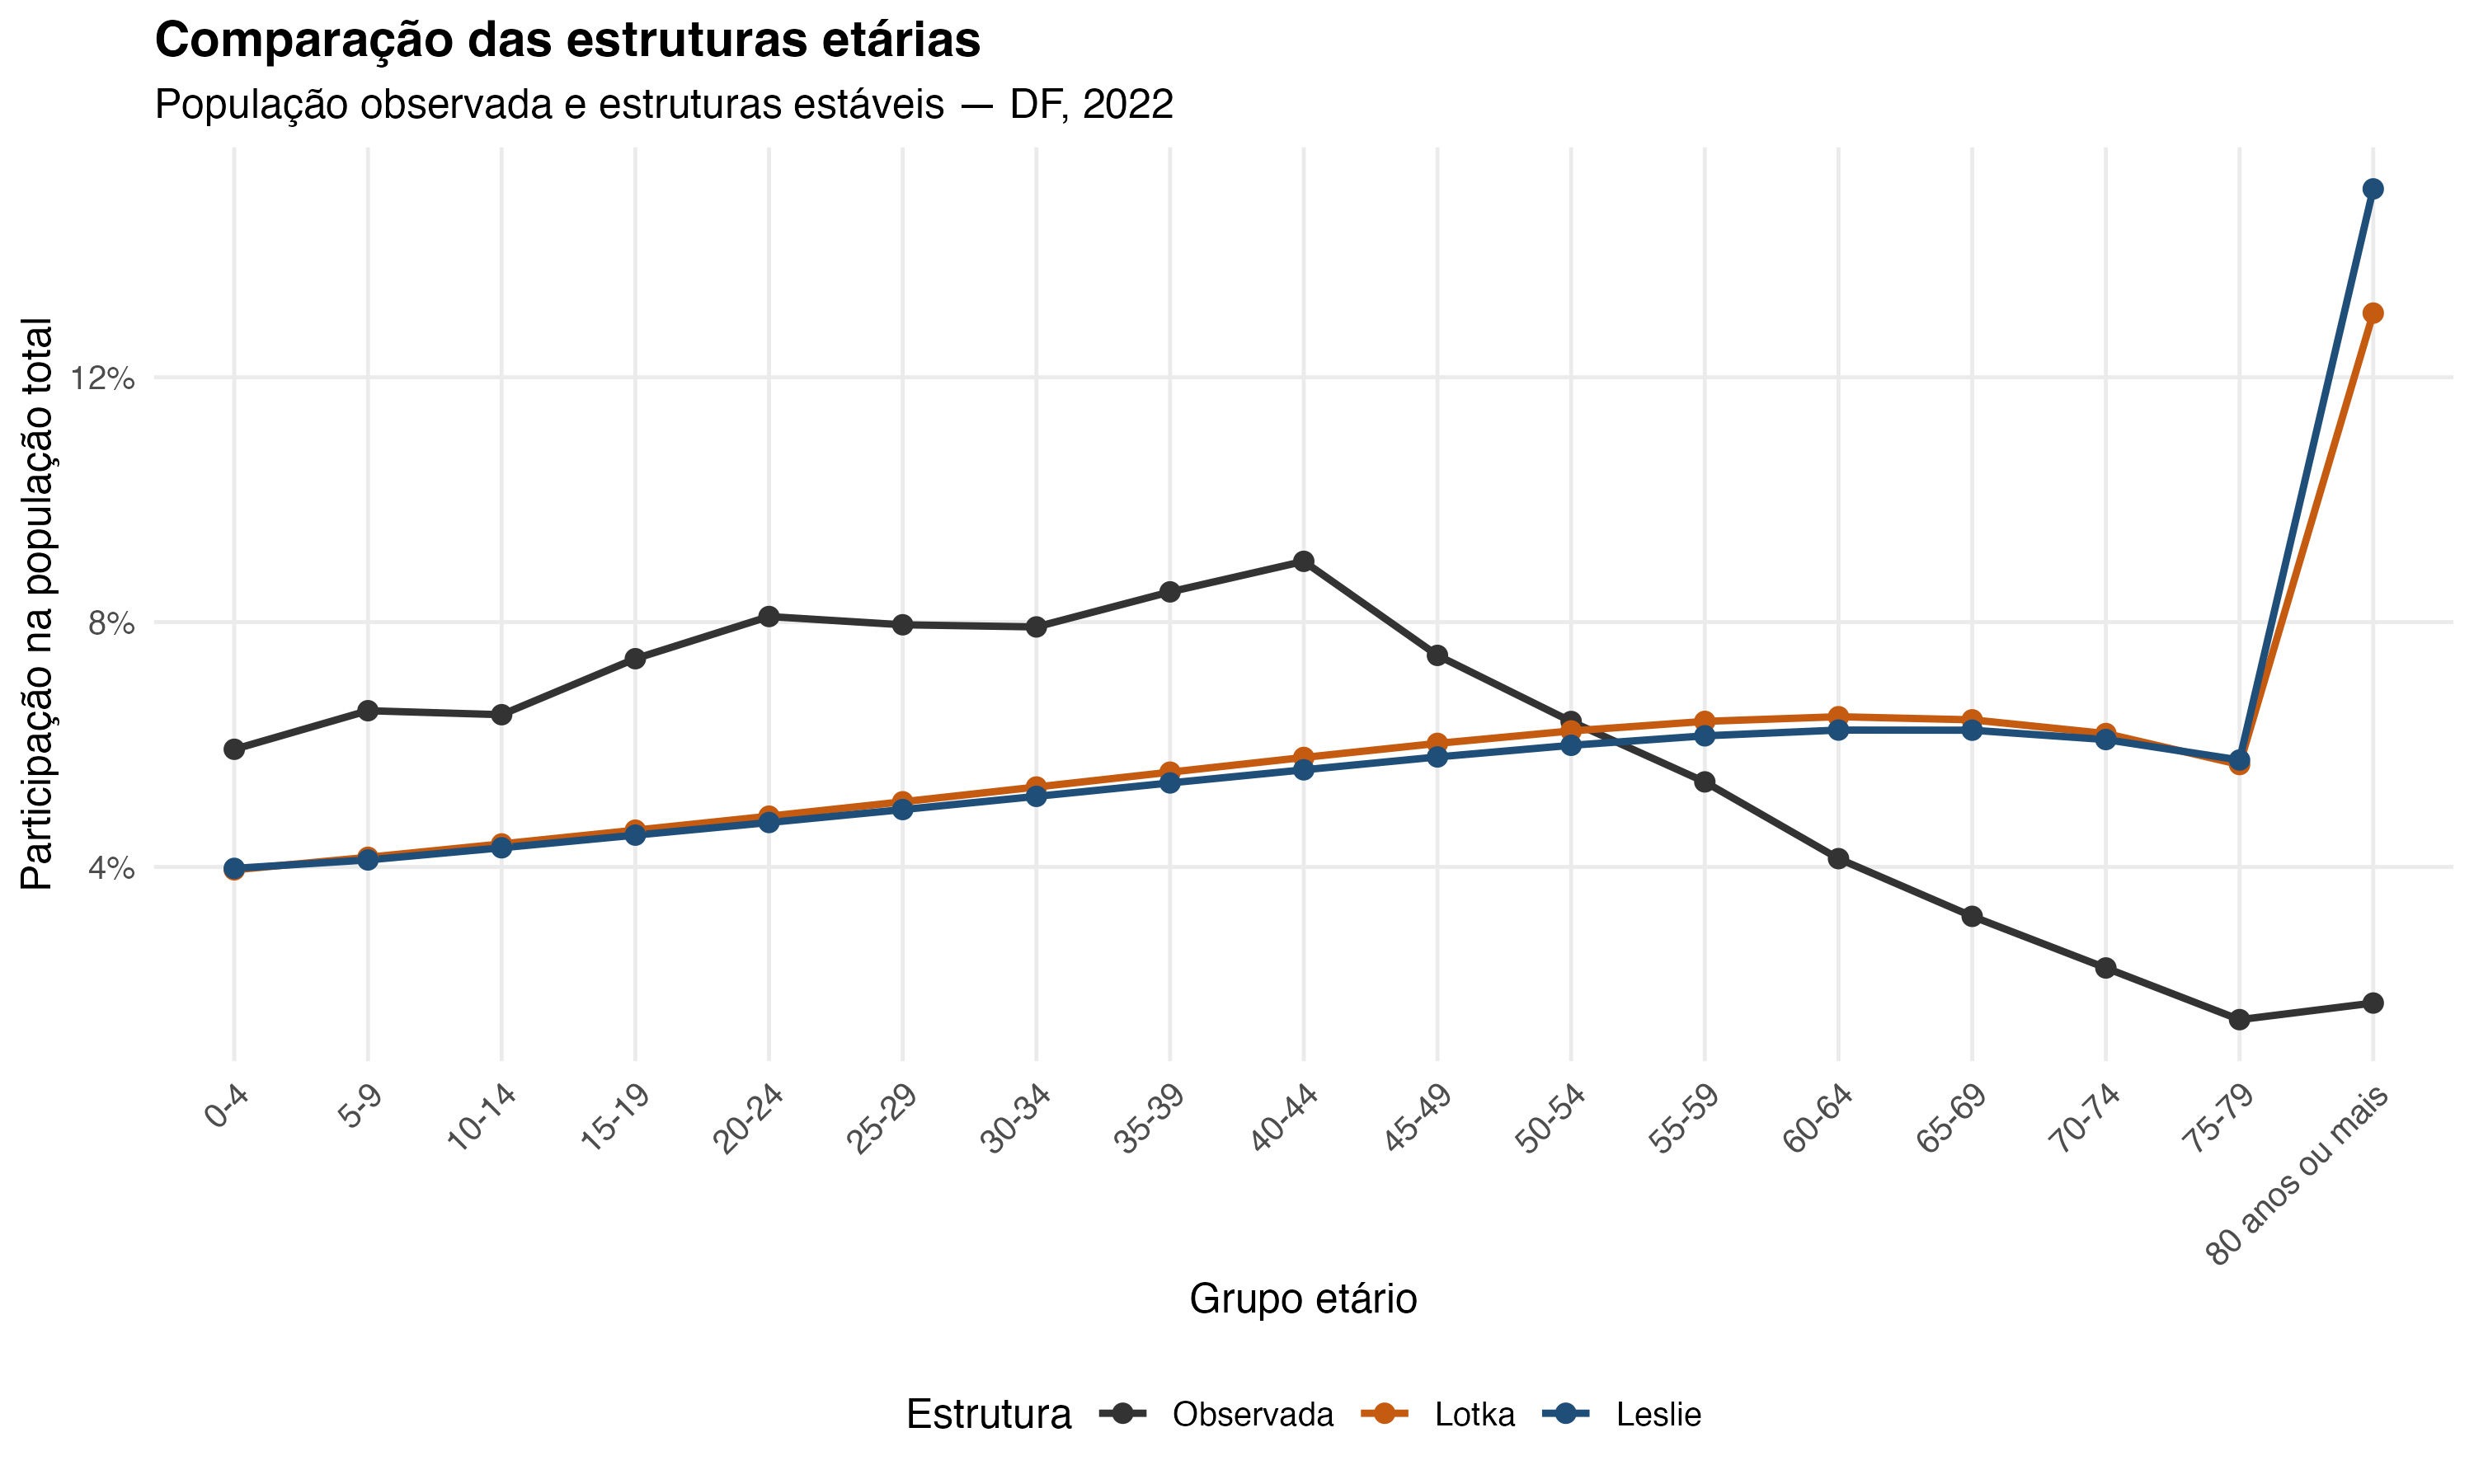
\includegraphics[width=0.94\textwidth]
{../figuras/comparacao_estruturas_etarias_df_2022.png}
\caption{Comparação entre a estrutura etária observada e as estruturas estáveis estimadas}
\label{fig:comparacao_estruturas}
\vspace{0.2cm}
\fonte{Elaboração própria com dados do Censo Demográfico, SINASC e SIM de 2022.}
\end{figure}

As estimativas obtidas pelos dois métodos são próximas, sobretudo até o grupo de 75 a 79 anos. Ambas apresentam menor participação de crianças e adultos e maior concentração de idosos do que a estrutura observada. A participação da população com 65 anos ou mais aumenta de 8,82\% na estrutura observada para 31,30\% na formulação de Lotka e 33,14\% na formulação matricial. Simultaneamente, a participação das pessoas de 0 a 14 anos diminui de 18,96\% para aproximadamente 12,4\%.

Essas diferenças indicam que a estrutura observada em 2022 ainda não corresponde àquela implícita nas condições correntes de fecundidade e mortalidade. Mantidas essas condições, e na ausência de migração, o envelhecimento populacional prosseguiria até a convergência para uma distribuição estável. A maior participação do grupo aberto de 80 anos ou mais nas estruturas estimadas também é influenciada pelo acúmulo dos sobreviventes nesse intervalo, devendo ser interpretada considerando o tratamento metodológico do grupo aberto.

As estruturas estáveis não constituem previsões da população futura do Distrito Federal. Elas representam resultados condicionais, obtidos sob a hipótese de manutenção indefinida das taxas demográficas de 2022 e de fechamento da população à migração \cite{grupofoz2021,preston2001}. A comparação deve, portanto, ser entendida como uma medida da distância entre a estrutura atual e aquela compatível com o regime demográfico analisado.


\section{Momentum populacional}

O momentum populacional corresponde à variação do tamanho da população que ocorre após a fecundidade atingir imediatamente o nível de reposição. Mesmo com crescimento assintótico nulo, a população pode continuar crescendo ou diminuir durante várias décadas, pois sua trajetória depende da estrutura etária existente no início da transição. Uma população com elevada concentração de pessoas nas idades reprodutivas, por exemplo, pode produzir gerações numerosas antes de alcançar uma estrutura estacionária \cite{grupofoz2021,preston2001}.

Para estimar o momentum do Distrito Federal, a fecundidade feminina de 2022 foi multiplicada por um fator de ajuste igual a 1,360947, determinado numericamente para que o autovalor dominante da matriz fosse igual a um. Assim, o crescimento assintótico do cenário é nulo. A mortalidade foi mantida constante, a migração foi fixada em zero e a população observada em 2022 foi utilizada como vetor inicial. A população foi então projetada iterativamente pela matriz até a convergência para uma estrutura estacionária.

O índice de momentum foi calculado por

\begin{equation}
M = \frac{N_{\infty}}{N_{2022}},
\end{equation}

\noindent em que $N_{2022}$ representa a população inicial e $N_{\infty}$ corresponde ao tamanho populacional após a estabilização.

\begin{table}[H]
\centering
\caption{Indicadores do momentum populacional, Distrito Federal, 2022}
\label{tab:momentum}
\begin{tabular}{lr}
\toprule
\textbf{Indicador} & \textbf{Valor} \\
\midrule
População inicial em 2022 & 2.817.381 \\
População máxima & 3.476.240 \\
Ano da população máxima & 2067 \\
Crescimento máximo em relação a 2022 & 23,39\% \\
População estacionária final & 3.427.140 \\
Índice de momentum & 1,2164 \\
Crescimento final em relação a 2022 & 21,64\% \\
Ano aproximado de estabilização & 2532 \\
\bottomrule
\end{tabular}

\vspace{0.2cm}
\fonte{Elaboração própria com dados do Censo Demográfico, SINASC e SIM de 2022.}


\end{table}

\begin{figure}[H]
\centering
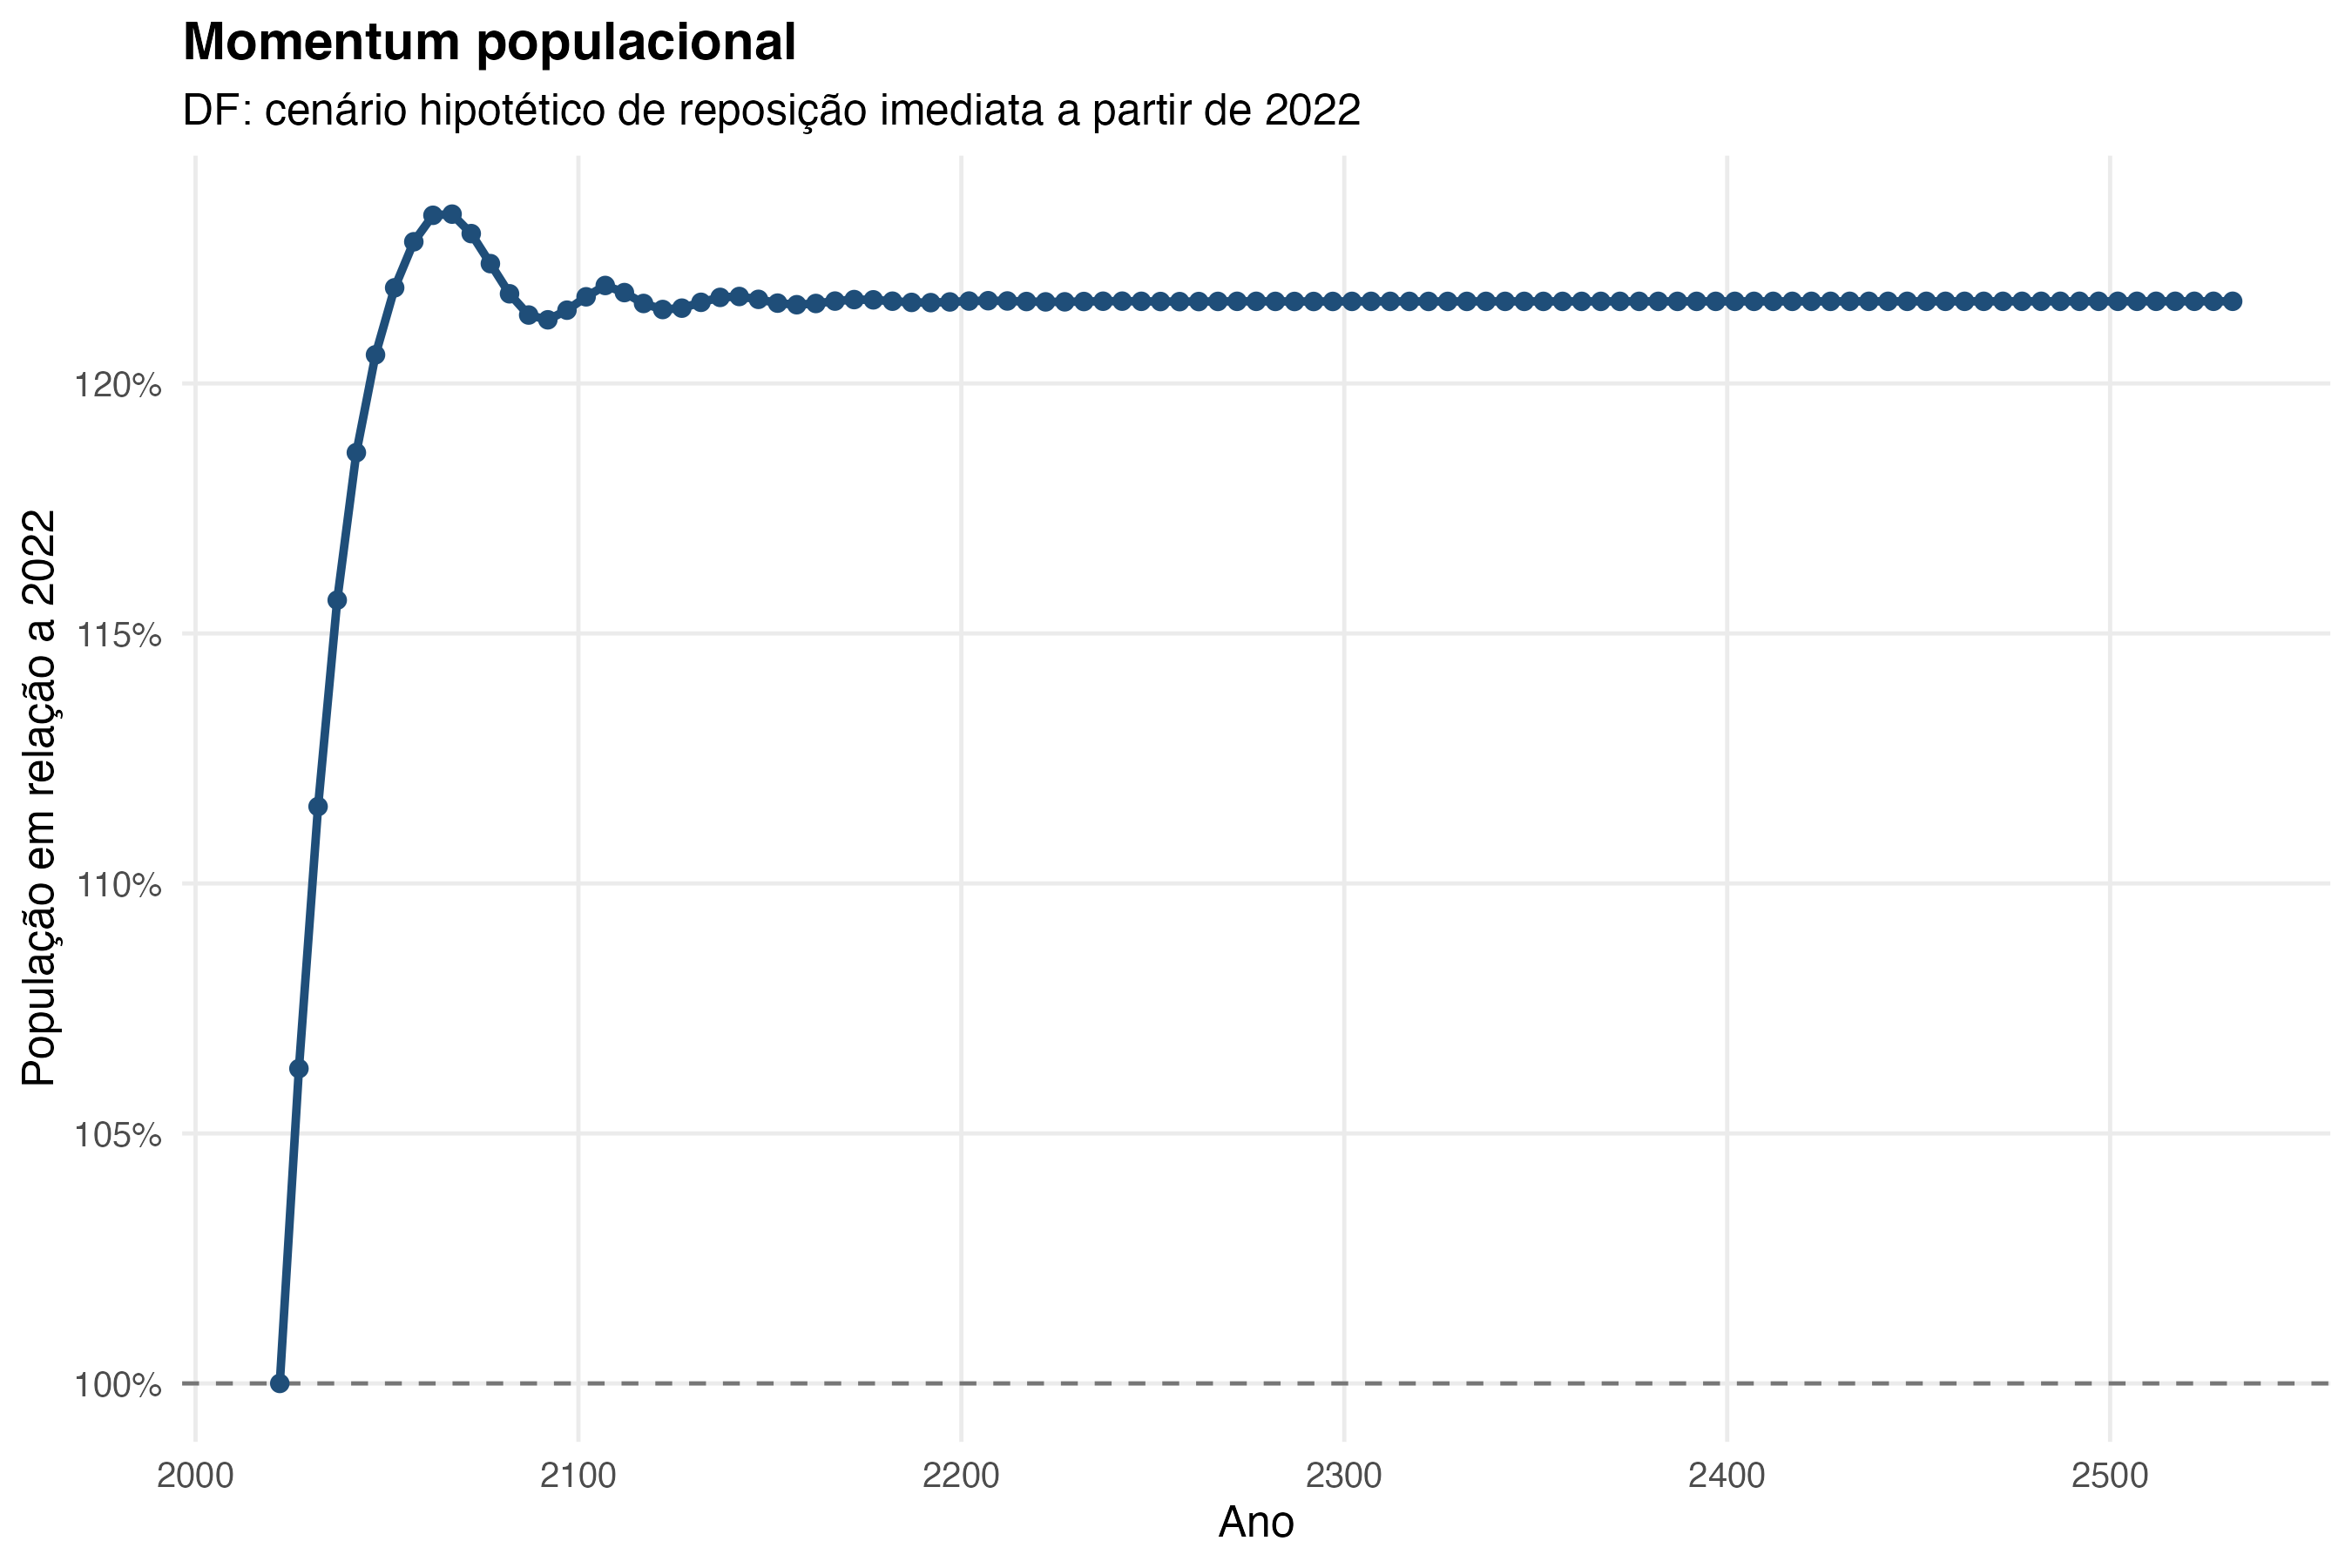
\includegraphics[width=0.94\textwidth]
{../figuras/momentum_populacional_df_2022.png}
\caption{Trajetória do momentum populacional, Distrito Federal, 2022}
\label{fig:momentum}
\vspace{0.2cm}
\fonte{Elaboração própria com dados do Censo Demográfico, SINASC e SIM de 2022.}
\end{figure}

Os resultados indicam que, mesmo se a fecundidade fosse ajustada imediatamente ao nível de 
reposição em 2022, a população do Distrito Federal ainda apresentaria crescimento. A população 
aumentaria de 2,817 milhões para um máximo de 3,476 milhões em 2067, equivalente a um 
crescimento de 23,39\%. Após esse ponto, ocorreria uma redução moderada até a convergência 
para aproximadamente 3,427 milhões de habitantes.

O índice de momentum de 1,2164 indica que a população estacionária seria 21,64\% maior que a 
população observada em 2022. A diferença entre o máximo transitório e o valor estacionário 
decorre do ajuste gradual da composição etária ao novo regime de fecundidade. O ano de 2532 
representa o atendimento ao critério numérico de convergência adotado, e não uma previsão 
pontual da data em que a população do Distrito Federal efetivamente se estabilizará.

Portanto, o crescimento residual estimado resulta exclusivamente da estrutura etária inicial. Os valores não constituem uma projeção populacional, pois pressupõem fecundidade de reposição imediata, mortalidade constante e ausência de migração durante todo o período.


\section{Considerações finais}

Este trabalho estimou indicadores de reprodução e população estável para o Distrito Federal com 
base nas condições demográficas de 2022. Os resultados mostram um padrão de fecundidade 
concentrado entre 25 e 34 anos, com idade média à maternidade de 29,37 anos. A Taxa Bruta de 
Reprodução foi estimada em 0,7506 filha por mulher e a Taxa Líquida de Reprodução em 0,7336, 
indicando que, sob as condições observadas, uma geração de mulheres não seria integralmente 
substituída pela geração seguinte.

A taxa intrínseca de crescimento foi negativa nos dois procedimentos empregados. A aproximação 
baseada na TLR resultou em $100r=-1,0562\%$ ao ano, enquanto a solução da equação de Euler--Lotka 
produziu $-1,0474\%$ ao ano. A proximidade entre as estimativas indica que a aproximação pela 
duração média da geração, estimada em 29,33 anos, representou adequadamente o regime reprodutivo 
analisado. A taxa bruta de natalidade da população estável foi estimada em 7,80 nascimentos por 
mil habitantes.

As estruturas estáveis obtidas pelas formulações de Euler--Lotka e matricial foram semelhantes e consideravelmente mais envelhecidas que a estrutura observada. Enquanto a população com 65 anos ou mais representava 8,82\% da população recenseada, sua participação alcançou 31,30\% na estrutura de Lotka e 33,14\% na estrutura matricial. Esses resultados mostram que a composição etária observada em 2022 ainda não refletia integralmente os efeitos de longo prazo da fecundidade abaixo do nível de reposição.

A simulação de reposição imediata produziu um índice de momentum igual a 1,2164. Com o autovalor dominante ajustado para um, a população aumentaria de 2,817 milhões de habitantes para um máximo de 3,476 milhões em 2067 e convergiria posteriormente para aproximadamente 3,427 milhões. Portanto, a estrutura etária inicial permitiria um crescimento residual de 21,64\% até a estabilização.

Os resultados são condicionais às hipóteses dos modelos: manutenção das taxas de fecundidade e mortalidade, ausência de migração e regularidade dos padrões por idade. Essas condições são especialmente restritivas para o Distrito Federal, cuja estrutura populacional é influenciada por movimentos migratórios. Assim, as estimativas não devem ser interpretadas como previsões, mas como medidas sintéticas das implicações de longo prazo do regime demográfico de 2022. Em conjunto, os indicadores apontam para uma dinâmica de baixa reprodução, crescimento intrínseco negativo e acentuado envelhecimento potencial da população.



{\singlespacing
\clearpage
\bibliography{references}
}
\end{document}
